\documentclass[letterpaper,12pt]{article} 
\usepackage[utf8]{inputenc}
\usepackage[dvipsnames]{xcolor}
\usepackage[colorlinks=true,urlcolor=ForestGreen]{hyperref}
\usepackage{titlesec}
\usepackage[margin=1in]{geometry}
\usepackage{longtable}
\usepackage{enumitem}
\usepackage{blindtext}
\usepackage{graphicx}
\usepackage{titlepic}
\usepackage{xcolor}     % Used to select color of code sections
\usepackage{soul}       % Used to highlight code sections
\usepackage{rotating}   % Used for landscape figure
\usepackage{pdflscape}

%Setting images folder
\graphicspath{{images/}}

%Setting the font I want:
\renewcommand{\familydefault}{\sfdefault}
\renewcommand{\sfdefault}{ppl}

%Changing highlight color
\sethlcolor{lightgray}

%Defining the entry command:
\newcommand{\entry}[4]{
  \begin{minipage}[t]{.05\textwidth}
  \end{minipage}
  \hfill\vline\hfill
  \begin{minipage}[t]{.90\textwidth}
    {\bfseries#1} {\hfill\underline{\bfseries#2}}
    
    \textit{#3}
    
    {#4}
  \end{minipage}\\\vspace{.25cm}}

%Some macros because I'm lazy:
\newcommand{\unito}{University of Turin}
\newcommand{\code}[1]{\hl{\texttt{#1}}}
\newcommand{\github}{https://github.com/carlo-deintinis/circhunter}

%Section spacing and format:
\titleformat{\section}
{\bfseries\Huge\scshape\raggedright}
{}
{1em}
{\thesection \hspace{0.40in}}[\titlerule]
\titlespacing{\section}{0pt}{3pt}{3pt}

%Section spacing and format:
\titleformat{\subsection}
{\bfseries\Large\scshape\raggedright}
{}
{1em}
{\thesubsection \hspace{0.25in}}
\titlespacing{\subsection}{0pt}{3pt}{3pt}

%{\bfseries\raggedright}
%{}
%{0em}
%{}[ $\bullet$]
%\titlespacing{\subsection}{0pt}{1pt}{3pt}


% Table of contents color
\hypersetup{colorlinks=true, linkcolor=black}

\begin{document}

\title{CircHunter Manual}
\author{Carlo De Intinis}

\maketitle

\begin{center}

\includegraphics[width=\textwidth]{circhunter_logo.png}
\end{center}

\tableofcontents
\newpage

\section{System requirements}
\subsection{Docker installation}
CircHunter requires the free version of the program Docker installed on the system. Depending on the user's installed Linux distribution, the installation process may be different. Please refer to the \textit{Get Docker} section of the Docker website (\href{http://www.docker.com}{www.docker.com}).

\subsection{Giving docker non-root access}

When docker is installed, it will be required to be given non-root access.

To do so, a docker group must be created (if it does not already exist):

\bigskip

\noindent\code{sudo groupadd docker}

\bigskip

Then, the connected user ``\$USER'' is added to the docker group.

\bigskip

\noindent\code{sudo gpasswd -a \$USER docker}

\bigskip

Run \code{newgrp docker} or log out and log in to activate the changes to groups. To check if the procedure was succesful, the command \code{docker run hello-world} should be executed.
 
\subsection{CircHunter installation}

The CircHunter software suite is contained inside a Docker repository that can be obtained running the following command:

\bigskip

\noindent\code{docker pull carlodeintinis/circhunter:latest}

\subsection{Launching CircHunter}

When the installation process is complete, it is possible to use the Command Line Interface (CLI) to execute the provided launcher script (circhunter.sh) with all the required arguments for the analysis. Alternatively, the CLI can be used to launch the CircHunter graphical interface contained in the provided jar file (CircHunterGUI.jar).

\bigskip

The CircHunter launcher script and graphical user interface can be downloaded from the GitHub repository \github.

On a system with git installed it is possible to download the repository by entering the command \code{git clone \hbox\github}.

\section{Input data}
\label{sec:input_data}
In this section, the requirements of input files to use with CircHunter are described in detail. However, as a general rule, all files must be in plain text (no encoded files).

\subsection{Circular RNA file}

The file containing circular RNA information must be composed of the following TAB separated columns:
\begin{itemize}
  \item chromosome name specified as chr\#\# (i.e. chr1, chr12)
  \item start position
  \item end position
  \item circRNA name specified as chr\#\#\_start\_end (i.e. chr1\_10\_100)
  \item genomic strand specified as 1 (forward) or -1 (reverse)
\end{itemize}
Every row of the file is used for a single circRNA, with EOL characters to distinguish circRNAs from one another.

\subsection{Genome file}
Three main genomes are officially supported by CircHunter: hg18, hg19 and hg38. Of these, \textbf{hg19} comes preinstalled, the others are downloaded by the program when they are requested via the argument \textit{-as}.

A downloaded genome or a not supported genome may be provided via the argument \textit{-sg}, however please note that CircHunter default behaviour is to remove every genome entry that does not comply with the accepted chromosome names (from chr1 to chr22, chrX and chrY).

All required genome data is shown in Table \ref{tab:genome_file}.

\begin{table}[h]
  \centering
  \begin{tabular}{l | p{7cm}}
    Label & Description\\
    \hline \hline
    ENSG & Ensembl Gene ID \\
    ENST & Ensembl Transcript ID \\
    ENSE & Ensembl Exon ID \\
    Chr & Chromosome name \\
    Exon chr start & Start position of exon \\
    Exon chr end & End position of exon \\
    Strand & Strand of exon (1 or -1) \\
    Exon Rank in Transcript & Rank of the exon \\
    Gene start & Start position of exon's gene \\
    Gene end & End position of exon's gene \\
    Transcript start & Start position of exon's transcript \\
    Transcript end & End position of exon's transcript \\
  \end{tabular}
  \caption{Genome exon export data requirements. All fields must be TAB separated.}
  \label{tab:genome_file}
\end{table}

\subsection{Isoform data file}

The isoform data file is used by CircHunter to obtain a unique classification of circRNAs. If this file is not provided, CircHunter will download the required data using an available internet connection. All required data is shown in Table \ref{tab:isoform_data_file}.

\begin{table}[h]
    \centering
    \begin{tabular}{l | l}
        Label & Description \\
        \hline \hline
        ENSG & Ensembl Gene ID \\
        ENST & Ensembl Transcript ID \\
        Chr & Chromosome name \\
        External transcript name & Isoform identifier \\
    \end{tabular}
    \caption{Isoform data file requirements. All fields must be TAB separated.}
    \label{tab:isoform_data_file}
\end{table}

\section{CLI usage}
CircHunter is launched via the script \textbf{circhunter.sh}, to which all the arguments for the execution of the analysis must be provided. The user must specify an \textit{execution mode} to select the type of analysis and some \textit{arguments} that are used to provide file locations and analysis options.

\subsection{Execution modes}
CircHunter relies on four main execution modes that can be invoked through specific flags. These modes are described below.

\vspace{0.25in}

\entry
{-c, - -classification}
{circRNA classification}
{Requires: -cr. \hspace{0.25in} Optional: -sg, -as, -id, -of }
{CircHunter will output a transcript-wise classification of the provided circRNAs. Outputs a file named \textit{circRNA\_classification} where every row represents a transcript associated with a circRNA and consequently the classification of that circRNA referring to the transcript. This mode also outputs a unique circRNA classification: every cirRNA is assigned to one particular classification, in order of importance. Refer to Section \ref{sec:circ_classification} for additional information regarding the classification process.}

\entry
{-s, - -sequences}
{circRNA backsplicing junction sequences}
{Requires: -cr \hspace{0.25in} Optional: -sg, -as, -of}
{CircHunter outputs the backsplicing junction sequences of all the provided circRNAs. The sequences' span is of +70/-70bp and all sequences are obtained considering the full genomic sequence (intronic sequences are not removed). Sequences are outputted in a FASTA format file named \textit{circRNA\_backsplicing\_sequences.fasta}.}

\entry
{-r, - -readcount}
{read count of backsplicing junction sequences}
{Requires: -rs, -bj \hspace{0.25in} Optional: -hc, -of}
{The HashCirc suite is executed. The RNA-Seq data is used in conjunction with the backsplicing junction sequences provided in order to obtain a count of the RNA-Seq reads that represent the backsplicing junction sequences. Of the two steps required, the first one may be parallelized modifying the appropriate \textit{-hc} value. Results are saved in multiple files named \textit{readcount}i where \textit{i} is the part number (determined by the parallelization process).}

\entry
{-f, - -full}
{full}
{Requires: -cr \hspace{0.25in}Optional: -sg, -as, -id, -of}
{CircHunter will execute the \textbf{circRNA classification} execution mode followed by the \textbf{circRNA backsplicing junction sequences} mode, allowing the user to obtain both results in a single step. Output files from both execution modes are obtained, with the same names specified above.}

\subsection{Arguments}

In addition to the execution mode, CircHunter can use the arguments described in this section. Please refer to Section \ref{sec:input_data} for additional information regarding required file contents and formats.

\vspace{0.25in}

\entry
{-h, - -help}
{help}
{}
{Shows a quick help screen in the CLI.}


\entry
{-cr, - -circrna}
{supplied circRNA list file}
{}
{File containing the coordinates of cirRNAs to investigate.}

\entry
{-sg, - -suppliedgenome}
{supplied exon export file}
{Supported genomes: hg18, hg19, hg38}
{File containing a Biomart exon export. CircHunter will filter out any export referring to non-canonical chromosome names. A specific set of genes instead of a full genome can be supplied. Please note that the hg19 genome comes pre-installed within the CircHunter's Docker environment, so it is not necessary to supply it if a genome-wide research is the researcher's goal.}

\entry
{-id, - -isoformdata}
{supplied gene isoform data}
{Supported genomes: hg18, hg19, hg38}
{File containing the isoform data required for the circRNA univocal classification process. If this data is not provided by the user, CircHunter will download it.}

\entry
{-rs, - -rnaseq}
{supplied RNA-Seq file}
{}
{RNA-Seq file supplied by the researcher. There is no need to split the file for parallelization purposes, this can be accomplished with the \textit{-hc} argument.}

\entry
{-bj, - -bksjunctions}
{supplied circRNA backsplicing junction sequences}
{}
{File containing the sequence that represents the circRNA backsplicing junctions. These sequences can be obtained from execution mode \textit{-s}.}

\entry
{-of, - -outputfolder}
{supplied output folder}
{Defaults to: $\sim$/CircHunter/data}
{Use this argument to specify a custom output folder.}

\entry
{-as, - -assembly}
{genome assembly to use for backsplicing sequences}
{Available choices: hg18, hg19 (default), hg38}
{CircHunter can use three different genomes. Of these, hg19 is the default and it is selected whenever \textit{-as} is missing. Also, hg19 is already installed in CircHunter's Docker environment, hg18 and hg38 can be provided by the user with the \textit{-sg} argument or can be downloaded autonomously by CircHunter during the analysis process. The download can require entire minutes, depending on the speed provided by the Biomart servers and the user connection.}

\entry
{-hc, - -hashcirc}
{arguments to pass to hashcirc}
{Syntax: -hc 1 2 3 4 5 6}
{Various arguments for the HashCirc step can be specified by the user. These arguments are listed below.
  \begin{enumerate}
    \item\textit{k}-mer size \quad $\bullet$ \quad \textit{k}-mer length (bp)
    \item thread number \quad $\bullet$ \quad Number of processes to parallelize (limited by CPU logic core number). 
    \item hash size \quad $\bullet$ \quad Dimensions of the hash table
    \item collision list size \quad $\bullet$ \quad Dimensions of the collision list
    \item\textit{k}-mer number \quad $\bullet$ \quad Number of \textit{k}-mers that must be matched to the sequence to consider the sequence itself as represented in the RNA-Seq data.
    \item matches \quad $\bullet$ \quad Number of perfect matches required in the \textit{k}-mer to consider it matched to a sequence.
  \end{enumerate}

}

\subsection{Extra functions}

\entry
{-cd, - -cleandocker}
{Clean docker images}
{Used to recover disk space}
{Every time CircHunter is launched, a Docker image is saved on the system. To recover the lost disk space, run this function with the following syntax: \code{bash circhunter.sh -cd}.}

\section{Syntax examples}

\noindent\code{bash circhunter.sh -c -cr circRNA\_file -as hg19}

CircHunter will execute \textbf{- -classification} mode and classify every circRNA in the \textit{circRNA\_file} that was provided by the user. The program will use the preinstalled \textit{hg19} genome. Isoform data and exon information are downloaded using an available internet connection.

\bigskip

\noindent\code{bash circhunter.sh -c -cr circRNA\_file -sg genome\_file -as hg19 -id isoform\_data\_file}

Same as above, but CircHunter uses the provided genome file and isoform data file instead of downloading the data.

\bigskip

\noindent\code{bash circhunter.sh -s -cr circRNA\_file -as hg19 -of path/outputfolder}

CircHunter executes \textbf{- -sequences} mode and obtains the backsplicing junction sequences of all circRNAs provided with the \textit{circRNA\_file}. A output folder has been provided with the \textbf{-of} argument (\textit{path/outputfolder}).

\bigskip

\noindent\code{bash circhunter.sh -f -cr circRNA\_file -as hg38 -sg genome\_file}

CircHunter executes \textbf{- -full} mode: the provided \textit{circRNA\_file} in conjunction with the provided genome (\textit{genome\_file}) are used to classify circRNAs and obtain the backsplicing junction sequences of the circRNAs.

\bigskip

\noindent\code{bash circhunter.sh -r -rs rnaseq\_file -bj backsplicing\_junction\_file -hc 27 3 100 10 5 6}

CircHunter will execute \textbf{- -rnaseq} mode and counts of the reads representing the provided circRNA backsplicing junctions will be obtained. The arguments necessary to hashcirc execution have been provided with the \textbf{-hc} argument.

\section{Graphical User Interface}
CircHunter presents a GUI that can be used to set an analysis process with ease. The GUI is packed in the file \textbf{CircHunterGUI.jar} and needs a java installation in order to run.

\bigskip

The gui can be launched via command line by moving to the folder containing the GUI file and entering the command \code{java -jar "CircHunterGUI.jar"}.

Alternatively the GUI can be launched from a file manager, but the file must be marked as executable by the user. This is done by entering the command \code{chmod+x CircHunterGUI.jar}.

\section{Toy Example}

CircHunter presents a toy example to test the correct execution of the program on the local machine. Figure \ref{fig:toyexample} shows a graphical representation of the fake circRNAs and genome features that are encoded in the example.

The example can be run by the user by entering the command below in the CLI. Please note that this command is valid in the main folder of CircHunter, otherwise the file paths must be adjusted by the user

\bigskip

\noindent\code{bash circhunter.sh -f -cr toyexample/toy\_circRNA -sg toyexample/toy\_genome -id toyexample/toy\_isoformdata -as hg19}

\bigskip

Table \ref{tab:toy_circrna} shows the circRNAs included in the toy example, whereas Table \ref{tab:toy_results} shows the expected result of the univocal classification process.

\begin{table}[h]
    \centering
    \begin{tabular}{c c c c c }
        chromosome & start pos. & end pos. & circRNA name & strand \\
        \hline\hline
        chr1 & 10 & 60 & chr1\_10\_60 & 1 \\
        chr1 & 70 & 90 & chr1\_70\_90 & 1 \\
        chr1 & 70 & 120 & chr1\_70\_120 & -1 \\
        chr1 & 100 & 160 & chr1\_100\_160 & 1 \\
        chr1 & 135 & 190 & chr1\_135\_190 & 1 \\
        chr1 & 165 & 195 & chr1\_165\_195 & 1 \\
    \end{tabular}
    \caption{circRNAs included in the toy example.}
    \label{tab:toy_circrna}
\end{table}

\begin{table}[h]
    \centering
    \begin{tabular}{l l c c}
        circRNA name & classification & isoform & isoform rank \\
        \hline\hline
        chr1\_100\_160 & intergenic & Isoform-001 & 001 \\
        chr1\_10\_60 & multiexon & Isoform-001 & 001 \\
        chr1\_135\_190 & intronic & OtherIsoform-001 & 001 \\
        chr1\_165\_195 & intronic & OtherIsoform-001 & 001 \\
        chr1\_70\_120 & multiexon & Isoform-201 & 201 \\
        chr1\_70\_90 & monoexon & Isoform-001 & 001 \\
    \end{tabular}
    \caption{Expected results of the \textbf{-f} run of the toy example data}
    \label{tab:toy_results}
\end{table}

\begin{landscape}
\begin{figure}[th]
    \centering
    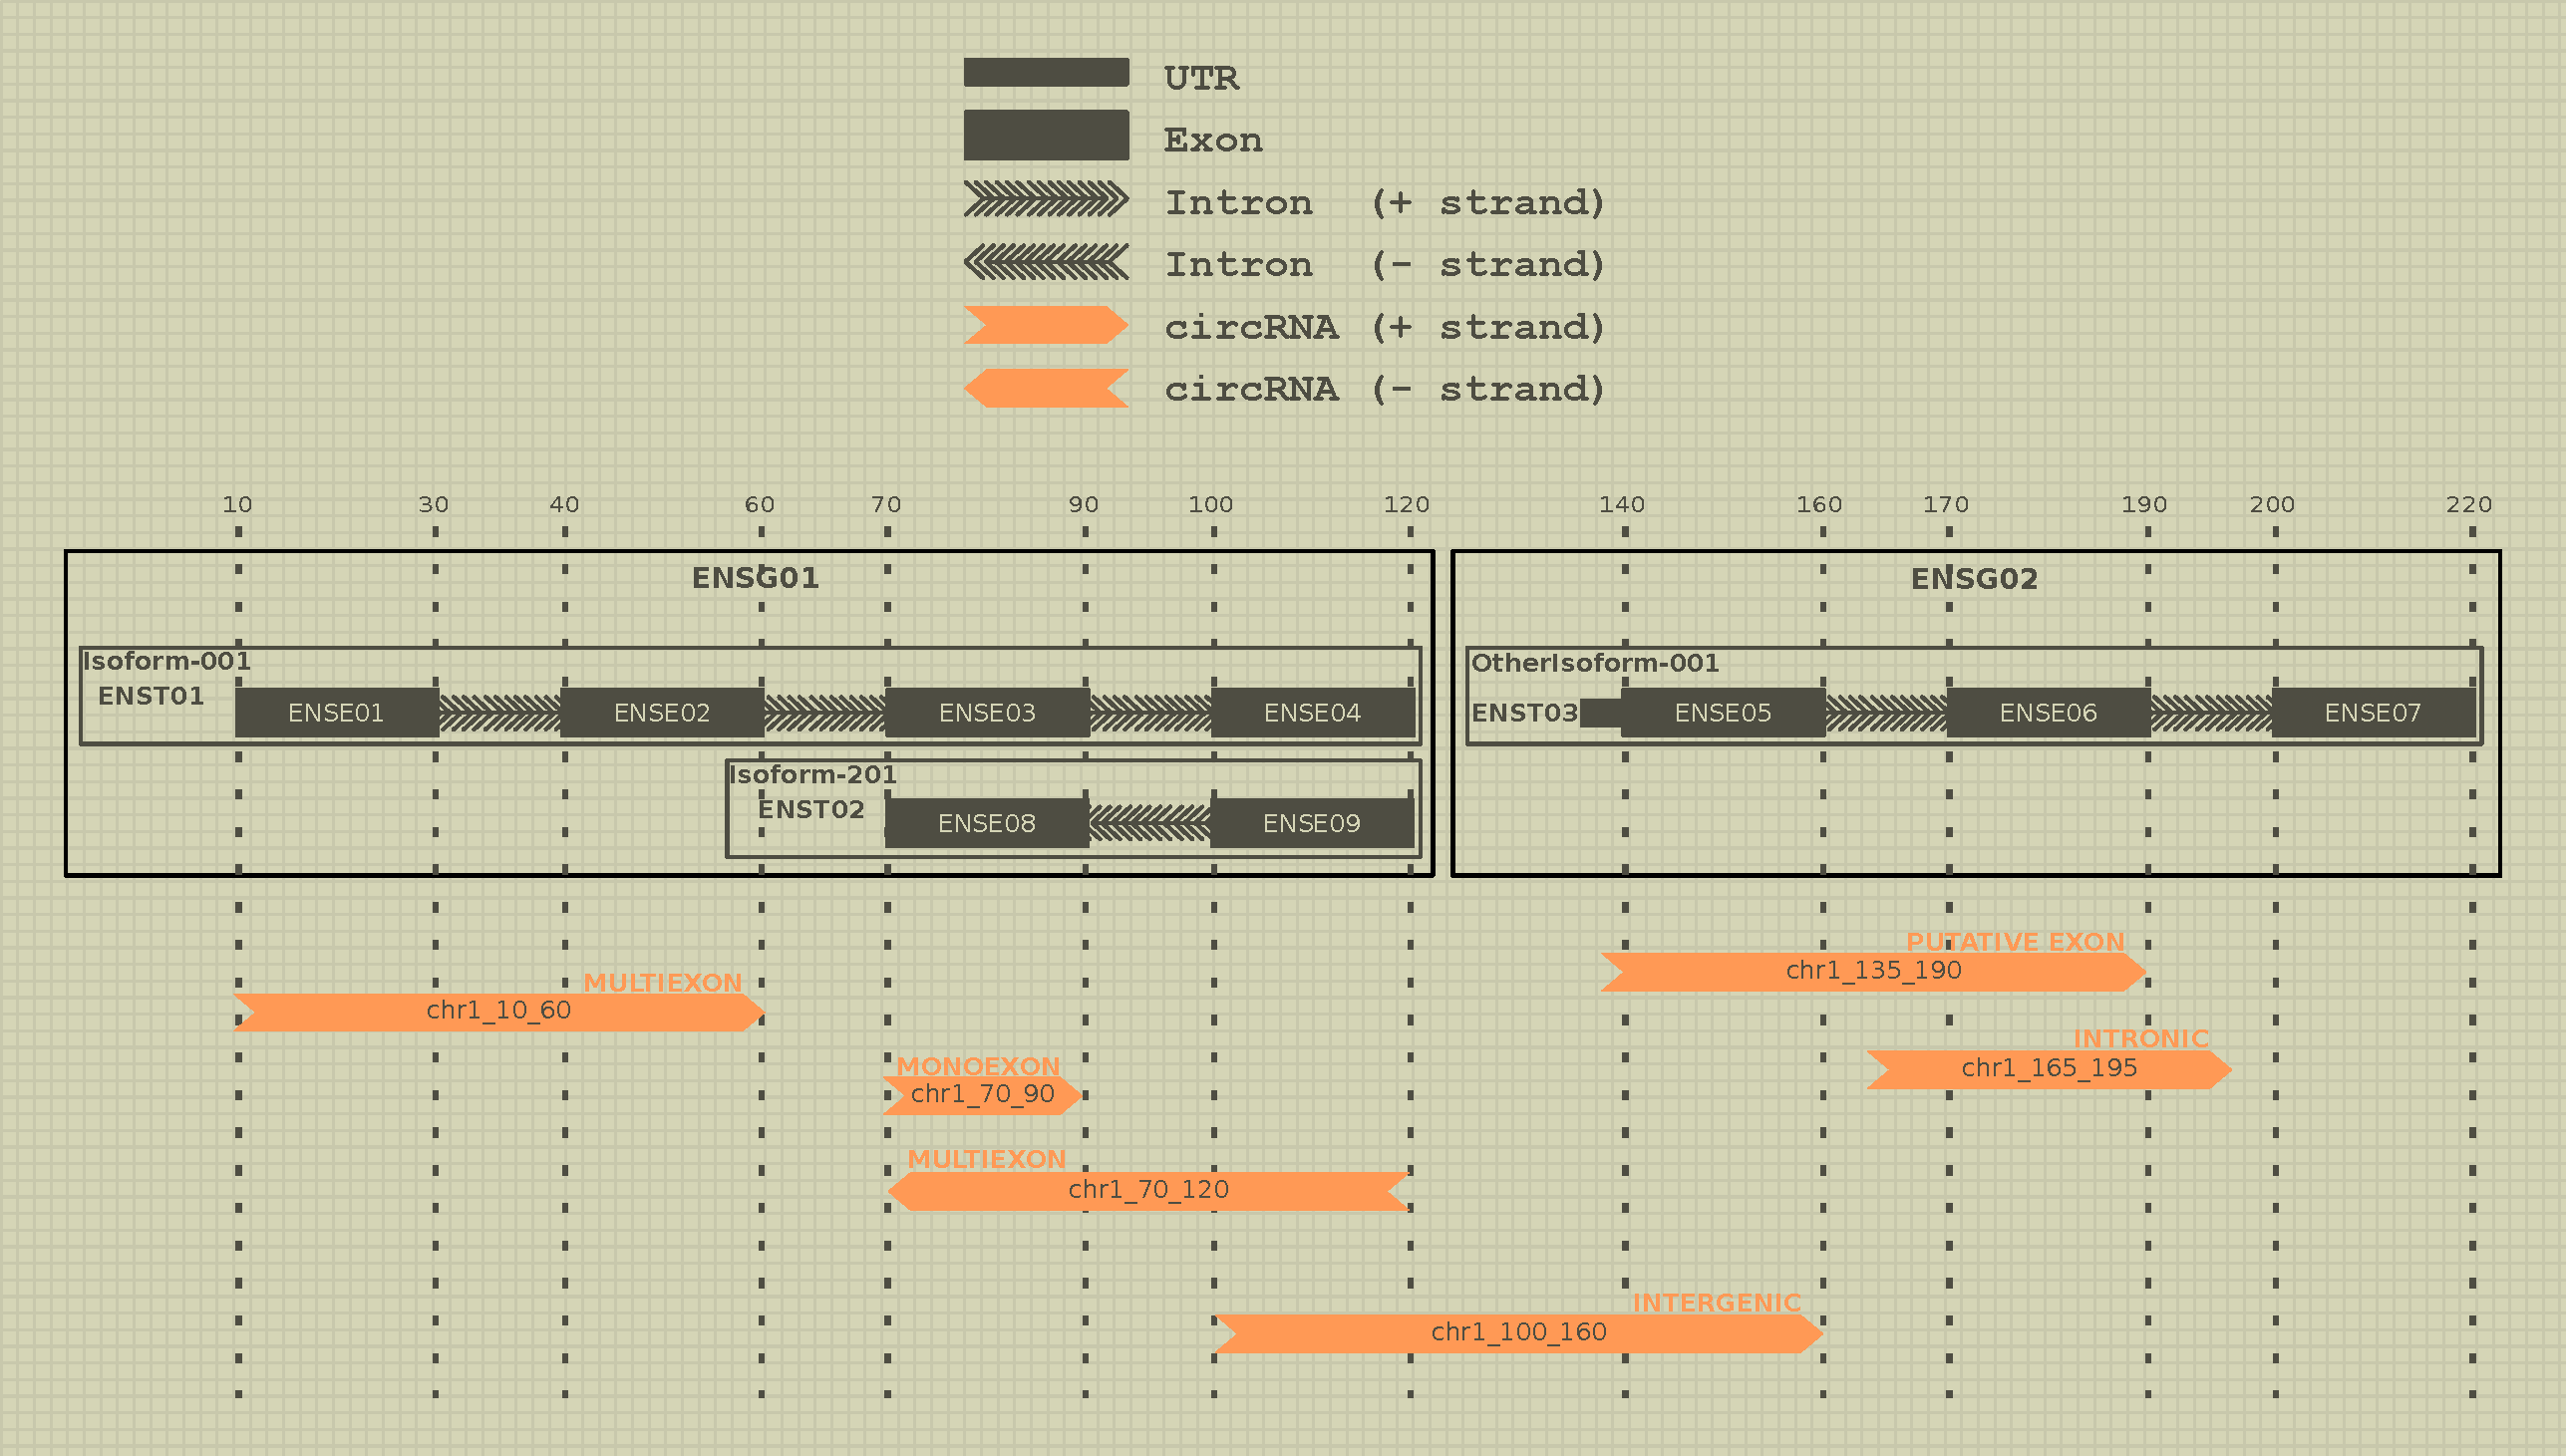
\includegraphics[scale=0.5]{toyexample.pdf}
    \caption{Representation of the example genome represented in the toy example files. The classification noted on the figure is the result of the univocal classification process of CircHunter. Note that the program is strand-aware and a circRNA won't align on the opposite strand.}
    \label{fig:toyexample}
\end{figure}
\end{landscape}

\end{document}
